\documentclass[12pt,a4paper]{article}

\usepackage{amsmath,amssymb}
\usepackage{graphicx}
\usepackage{hyperref}
\usepackage{natbib}
\usepackage{geometry}
\usepackage{booktabs}
\usepackage{float}
\usepackage{xcolor}
\usepackage{microtype}

\geometry{margin=1in}

\hypersetup{
  colorlinks=true,
  linkcolor=blue,
  citecolor=blue,
  urlcolor=blue
}

% ─────────────────────────────────────────────────────────────────────────────
\title{\textbf{Missing Satellites: The Virial Partition Closure Condition\\
and the Two Mechanisms}}

\author{Heath W.\ Mahaffey\\
\small Independent Researcher, Entiat, Washington 98822, USA\\
\small \href{mailto:hmahaffeyges@gmail.com}{hmahaffeyges@gmail.com}\\
\small \url{https://github.com/hmahaffeyges/IAM-Validation}}

\date{March 2026\\
\small Zenodo DOI: \href{https://doi.org/10.5281/zenodo.18702042}{10.5281/zenodo.18702042}}
% ─────────────────────────────────────────────────────────────────────────────

\begin{document}
\maketitle

% ─────────────────────────────────────────────────────────────────────────────
\begin{abstract}
The missing satellites problem --- the factor $\sim$8 discrepancy between the
$\sim$500 dark matter subhalos predicted by $\Lambda$CDM N-body simulations
and the $\sim$60 satellite galaxies observed around the Milky Way --- has
resisted a single unified physical explanation for over two decades. We
propose that the Informational Actualization Model (IAM) provides two
distinct mechanisms from one physical condition, both derivable from the
virial theorem for $1/r$ potentials without free parameters.

Mechanism~A operates at the perturbation level. IAM's matter-sector
gravitational coupling $\mu(a) < 1$, derived from the Landauer cost of
gravitational decoherence encoded on the cosmological horizon, suppresses
the late-time growth rate of structure. At $z = 0$, $\mu_0 = 0.864$,
corresponding to a 13.6\% suppression in the effective gravitational
coupling for matter. This prediction is tested against the full Planck~2018
likelihood through 17 converged MCMC chains yielding $\Delta\chi^2 = +0.54$
relative to $\Lambda$CDM with no free parameters. The suppression vanishes
at high redshift: $\mu \to 1$ as $\mathcal{E}(a) \to 0$ for $a \ll 1$.

Mechanism~B operates at the thermodynamic level. The virial theorem partitions
gravitational binding energy exactly in half at every scale: the geometric half
deposits into spacetime curvature; the informational half is the Landauer cost
of each quantum-to-classical transition and must be written to an available
encoding surface. Where no local black hole horizon can form, the virial
partition cannot close and the structure disperses. This condition predicts a
minimum velocity dispersion $\sigma_\mathrm{crit} \approx 4$~km\,s$^{-1}$
below which dark matter halos cannot virialize, consistent with the observed
absence of satellite galaxies below this threshold. The scaling
$M_\mathrm{min} \propto \sigma^3$ is a testable prediction distinct from the
$\sigma^2$ cusp-core relation and the $\sigma^4$ M--$\sigma$ relation. The
absolute normalization contains a systematic offset of $\sim$100$\times$,
identified as an open problem requiring the formal derivation of the
local-to-global encoding rate criterion.

Both mechanisms derive from a single physical condition: the virial theorem
$2K + V = 0$ requires both halves of the energy partition to close
simultaneously. The decisive test of Mechanism~A is Euclid DR1 (October 2026),
which will measure $\mu_0$ to $\sigma(\mu_0) \approx 0.04$ precision,
providing $3.4\sigma$ sensitivity to the predicted value. The decisive test of
Mechanism~B is a complete census of the satellite population below
$\sigma \approx 4$~km\,s$^{-1}$ with the Vera Rubin Observatory.
\end{abstract}

% ─────────────────────────────────────────────────────────────────────────────
\section{Introduction}
\label{sec:intro}
% ─────────────────────────────────────────────────────────────────────────────

The missing satellites problem was identified independently by
\citet{Klypin1999} and \citet{Moore1999}. High-resolution N-body simulations
of $\Lambda$CDM predict of order 500 dark matter subhalos with circular
velocities $v_c > 10$~km\,s$^{-1}$ within the virial radius of a Milky
Way-mass host. The observed population of satellite galaxies numbers
approximately 60, including the classical dwarfs discovered prior to SDSS and
the faint dwarfs identified in modern photometric surveys
\citep{Koposov2008, Tollerud2008}. Proposed explanations within $\Lambda$CDM
include reionization suppressing gas cooling in low-mass halos
\citep{Bullock2000, Benson2002}, ram pressure and tidal stripping removing
baryons from satellites \citep{Mayer2006}, and baryonic feedback ejecting gas
and reducing dark matter densities \citep{Read2005, Pontzen2012}. These
mechanisms operate on baryons; they do not address the underlying question of
whether the dark matter subhalo population itself is suppressed.

IAM~\citep{IAM_theory,IAM_obs} proposes a different origin. The suppression
of satellite counts is a consequence of the thermodynamic structure of
gravitational decoherence: the same process that generates dark energy at
cosmological scales produces a modification of the effective gravitational
coupling for matter at perturbation scales. This modification operates
directly on the dark matter subhalo population, not on the baryons within it.

This paper presents the two IAM mechanisms for the missing satellites problem
and derives their observational consequences. Section~\ref{sec:virial_closure}
establishes the virial partition closure condition from which
both mechanisms derive. Section~\ref{sec:mechA} presents Mechanism~A and its
MCMC validation. Section~\ref{sec:mechB} derives Mechanism~B and the
$\sigma_\mathrm{crit}$ prediction. Section~\ref{sec:unified} presents the
unified picture. Section~\ref{sec:tests} specifies the falsification criteria.

% ─────────────────────────────────────────────────────────────────────────────
\section{The Virial Partition Closure Condition}
\label{sec:virial_closure}
% ─────────────────────────────────────────────────────────────────────────────

For any bound system governed by a $1/r$ potential, the virial theorem states:
\begin{equation}
2K + V = 0, \qquad K = \tfrac{1}{2}|V|.
\label{eq:virial}
\end{equation}
This is an exact mathematical theorem, not an approximation, valid for
gravitational and Coulomb potentials at every scale from hydrogen atoms to
galaxy clusters.

Within IAM~\citep{IAM_theory}, the two halves of
Equation~\ref{eq:virial} correspond to two distinct physical channels. The
potential half $|V|/2$ deposits into spacetime curvature --- the geometric
channel described by general relativity. The kinetic half $K = |V|/2$ is the
Landauer cost~\citep{Landauer1961,IAM_thermo_virial} of the quantum-to-classical transition at
each virialization event: the thermodynamic price of writing classical
information permanently to an encoding surface at cost $k_B T \ln 2$ per
bit~\citep{Jacobson1995, CaiKim2005}.

Both halves must close simultaneously. The geometric half stabilizes in
spacetime curvature only when the informational half is absorbed by an
available encoding surface. This is the virial partition closure condition:
both channels must operate for classical structure to persist. A structure
that cannot close its informational channel cannot persist as classical
structure.

The cosmological coupling constant follows immediately from
Equation~\ref{eq:virial}:
\begin{equation}
\beta_m = \frac{\Omega_m}{2} = 0.1575,
\label{eq:beta}
\end{equation}
the fraction of matter energy density participating in decoherence per Hubble
time, derived from the virial theorem with zero free parameters. The
Planck~2018 MCMC posterior returns $\beta_m = 0.1583 \pm 0.0033$, consistent
with the virial prediction at $0.2\sigma$~\citep{IAM_obs}.

% ─────────────────────────────────────────────────────────────────────────────
\section{Mechanism A: Growth Suppression from $\mu < 1$}
\label{sec:mechA}
% ─────────────────────────────────────────────────────────────────────────────

\subsection{Derivation}

The accumulated Landauer cost of all gravitational decoherence events since
the electroweak transition is measured by the activation
function~\citep{IAM_theory}:
\begin{equation}
\mathcal{E}(a) = \exp\!\left(1 - \frac{1}{a}\right),
\label{eq:Ea}
\end{equation}
where $a$ is the cosmological scale factor normalized to unity today.
$\mathcal{E}(a)$ is derived from horizon thermodynamics via the
Jacobson--Cai-Kim formalism~\citep{Jacobson1995,CaiKim2005}, not postulated.
It satisfies $\mathcal{E}(a) \to 0$ as $a \to 0$ and $d\mathcal{E}/da > 0$
always: the ledger only accumulates.

Photons travel null geodesics with $d\tau = 0$. They do not accumulate proper
time and do not participate in gravitational decoherence. The informational
modification applies exclusively to the matter sector. The effective
matter-sector gravitational coupling is:
\begin{equation}
\mu(a) = \frac{H^2_{\Lambda\mathrm{CDM}}}{H^2_{\Lambda\mathrm{CDM}}
+ \beta_m\,\mathcal{E}(a)},
\label{eq:mu}
\end{equation}
with $\beta_m = \Omega_m/2$ from Equation~\ref{eq:beta} and $\Sigma(a) = 1$
exactly for photons~\citep{IAM_obs}. At $z = 0$:
\begin{equation}
\mu(z{=}0) = \frac{1}{1 + \beta_m} = \frac{1}{1 + \Omega_m/2} = 0.864,
\label{eq:mu0}
\end{equation}
a 13.6\% suppression of the effective gravitational coupling for matter
(equivalently, $\mu_0 \equiv \mu(z{=}0) - 1 = -0.136$). At
high redshift, $\mathcal{E}(a) \to 0$ and $\mu \to 1$: the suppression is
a late-time effect. IAM predicts $\Lambda$CDM behavior at $z \gtrsim 2$.

The matter perturbation equation acquires an additional Hubble friction term:
\begin{equation}
\ddot{\delta}_m + 2H\dot{\delta}_m
- \frac{3}{2}\Omega_m H^2\,\mu(a)\,\delta_m = 0.
\label{eq:perturb}
\end{equation}
The suppression of $\delta_m$ at late times directly reduces the abundance
of virialized dark matter halos at the low-mass end of the mass function,
where the threshold for virialization is most sensitive to the growth rate.

\subsection{Quantitative suppression of the halo mass function}

The fractional change in the linear growth factor $D(z)$ between IAM and
$\Lambda$CDM at $z = 0$ is:
\begin{equation}
\frac{\Delta D}{D}\bigg|_{z=0}
= \frac{D_\mathrm{IAM}(0) - D_{\Lambda\mathrm{CDM}}(0)}
       {D_{\Lambda\mathrm{CDM}}(0)} \approx -0.074,
\label{eq:growth}
\end{equation}
a 7.4\% suppression in the linear growth factor~\citep{IAM_obs}. Via the
Press--Schechter formalism~\citep{PressSchechter1974}, the abundance of halos
of mass $M$ scales as $dn/dM \propto \exp(-\delta_c^2/2\sigma_M^2)$, where
$\sigma_M$ is the rms linear density fluctuation on scale $M$ and $\delta_c
\approx 1.686$ is the collapse threshold. A 7.4\% suppression in $D$ reduces
$\sigma_M$ proportionally. For halos near the satellite mass scale
$M \sim 10^7$--$10^9\,M_\odot$, where the exponential factor is sensitive
to small changes in $\sigma_M$, this produces a suppression in the predicted
satellite count that operates directly on the dark matter subhalo population,
independent of baryonic processes.

\subsection{MCMC validation}

Seventeen MCMC chains were run against the full Planck~2018 likelihood
\citep{PlanckVI2020} using MGCAMB~\citep{Hojjati2011} and
Cobaya~\citep{Torrado2021}. All 17 chains converged to $R-1 < 0.01$ with no
discarded runs and no parameter adjustments. The IAM-specific results
are~\citep{IAM_obs}:

\begin{table}[H]
\centering
\small
\caption{IAM MCMC results from 17 converged chains against Planck~2018.
All parameters fixed by virial theorem; no free parameters beyond
$\Lambda$CDM.}
\label{tab:mcmc}
\begin{tabular}{lll}
\toprule
Parameter & IAM posterior & Reference \\
\midrule
$\beta_m$ & $0.1583 \pm 0.0033$ & Virial prediction: $0.1577$ ($0.2\sigma$) \\
$\sigma_8$ & $0.7998 \pm 0.0058$ & KiDS-Legacy, DES~Y3, HSC~Y3 ($0.1\sigma$) \\
$H_0^\mathrm{(photon)}$ & $67.16 \pm 0.47$ km\,s$^{-1}$\,Mpc$^{-1}$ & Planck~2018 ($0.37\sigma$) \\
$H_0^\mathrm{(matter)}$ & $72.26$ km\,s$^{-1}$\,Mpc$^{-1}$ & SH0ES ($0.75\sigma$) \\
$\Delta\chi^2$ & $+0.54$ & vs $\Lambda$CDM best fit \\
\bottomrule
\end{tabular}
\end{table}

The predicted $\sigma_8 = 0.7998 \pm 0.0058$ is consistent with weak lensing
surveys at $0.1\sigma$. The suppression of $\sigma_8$ relative to the
Planck+$\Lambda$CDM value ($\sigma_8 \approx 0.811$) directly corresponds to
reduced small-scale power at the satellite mass scale.

% ─────────────────────────────────────────────────────────────────────────────
\section{Mechanism B: The Dispersal Condition}
\label{sec:mechB}
% ─────────────────────────────────────────────────────────────────────────────

\subsection{Physical origin}

The virial theorem requires both halves of the virial partition to
close simultaneously. The informational half --- the Landauer cost of each
quantum-to-classical transition --- must be written to an available encoding
surface. Two surfaces are available: the cosmological apparent horizon and a
local black hole horizon.

The cosmological apparent horizon is always present, but it is cold
($T_H = \hbar H/2\pi k_B \approx 2.66 \times 10^{-30}$~K at $z = 0$) and
expands uniformly, indifferent to individual localities. For a collapsing halo
with dynamical timescale $t_\mathrm{dyn} \ll H^{-1}$, the information
produced locally during collapse cannot be absorbed by the cosmic horizon fast
enough: the horizon is causally present but thermodynamically inadequate on
collapse timescales. A local hot encoding surface is required.

The black hole horizon is that surface. It forms when the accumulated
informational entropy from local gravitational decoherence saturates the
Bekenstein--Hawking bound on the bounding surface~\citep{IAM_BH}:
\begin{equation}
S_\mathrm{info}(R) \geq \frac{A(R)}{4\ell_P^2}.
\label{eq:saturation}
\end{equation}
Once formed, the black hole absorbs the informational half permanently. Where
this condition cannot be satisfied --- where the halo is not sufficiently
massive or compact --- the informational half of the virial partition is
produced but has no local surface to write to. The partition cannot close. The
halo disperses.

\subsection{Derivation of $M_\mathrm{min}$}

A collapsing halo of mass $M$ and velocity dispersion $\sigma$ has dynamical
timescale:
\begin{equation}
t_\mathrm{dyn} = \sqrt{\frac{\pi}{6G\rho}},
\label{eq:tdyn}
\end{equation}
where the mean density $\rho$ within the virial radius $r_v$ follows from the
virial relation. For a virialized halo, $v_c^2 = GM/r_v$ and
$\sigma^2 \approx v_c^2/2$, giving $\rho \propto \sigma^6/(G^3 M^2)$.
Substituting:
\begin{equation}
t_\mathrm{dyn} \approx \frac{\sqrt{\pi/6}\,GM}{\sigma^3}.
\label{eq:tdyn2}
\end{equation}
The condition $t_\mathrm{dyn} = H^{-1}$ identifies the boundary at which the
collapse timescale equals the cosmic expansion timescale. Below this boundary,
collapse is rapid enough that local decoherence production outpaces the cosmic
horizon's absorption capacity, and a local black hole vault is required. Setting
$t_\mathrm{dyn} = H^{-1}$ and evaluating at $z = 0$ where
$H_0 = H_0\sqrt{\Omega_m + \Omega_\Lambda} \approx H_0$ for the flat
Planck~2018 cosmology ($\Omega_m + \Omega_\Lambda = 1.0002$):
\begin{equation}
\boxed{M_\mathrm{min} = \frac{4\,\Omega_m\,\sigma^3}{G\,H_0}},
\label{eq:Mmin}
\end{equation}
with zero free parameters beyond $\Omega_m$ and $H_0$, both fixed by
Planck~2018 \citep{PlanckVI2020}: $\Omega_m = 0.3153$,
$H_0 = 67.36$~km\,s$^{-1}$\,Mpc$^{-1}$.

\subsection{The $\sigma_\mathrm{crit}$ threshold}

The observed halo occupation fraction drops sharply below
$M \approx 10^{8.4}\,M_\odot$~\citep{Kim2021}. Setting
$M_\mathrm{min}({\sigma_\mathrm{crit}}) = 10^{8.4}\,M_\odot$ in
Equation~\ref{eq:Mmin}:
\begin{equation}
\sigma_\mathrm{crit}
= \left(\frac{G\,H_0\,M_\mathrm{min}}{4\,\Omega_m}\right)^{1/3}
\approx 4\ \mathrm{km\,s}^{-1}.
\label{eq:sigma_crit}
\end{equation}
Below $\sigma_\mathrm{crit}$, the virial partition cannot close and no
satellite galaxy forms. Halos in this regime are not missing from the
predicted population; they disperse before becoming galaxies.

The $\sigma^3$ scaling of $M_\mathrm{min}$ is a testable prediction. It is
distinct from the $\sigma^2$ scaling of the cusp-core radius
$r_\mathrm{core} \propto \sigma^2$~\citep{IAM_small_scale} and the $\sigma^4$
scaling of the M--$\sigma$ relation~\citep{IAM_msigma}. All three derive from
the same thermodynamic identity~\citep{IAM_thermo_virial} at different boundary conditions; their
different power-law indices are a direct consequence of the different physical
regimes in which the virial partition closes.

\subsection{Honest accounting of the normalization}

The absolute normalization of Equation~\ref{eq:Mmin} contains a systematic
offset of $\sim$100$\times$ between the predicted and observed satellite masses.
Setting $M_\mathrm{min} = 10^{8.4}\,M_\odot$ yields
$\sigma_\mathrm{crit} \approx 4$~km\,s$^{-1}$, consistent with the observed
threshold; but the raw prediction from Equation~\ref{eq:Mmin} at
$\sigma = 4$~km\,s$^{-1}$ gives $M_\mathrm{min} \approx 10^{6.4}\,M_\odot$,
approximately 100$\times$ below the observed floor.

This offset is the same systematic identified in the cusp-core problem
(normalization offset $\sim$130$\times$, scaling confirmed)~\citep{IAM_small_scale}.
Both share the same physical origin: the local-to-global encoding rate
criterion --- the condition under which decoherence events are assigned to the
local black hole vault versus the global cosmic horizon --- has not yet been
formally derived. This is one open problem, not two. Its resolution will
simultaneously fix the normalization of $M_\mathrm{min}$ and the cusp-core
radius. The $\sigma^3$ scaling and the $\sigma_\mathrm{crit}$ threshold are
independent of this normalization.

\begin{figure}[H]
\centering
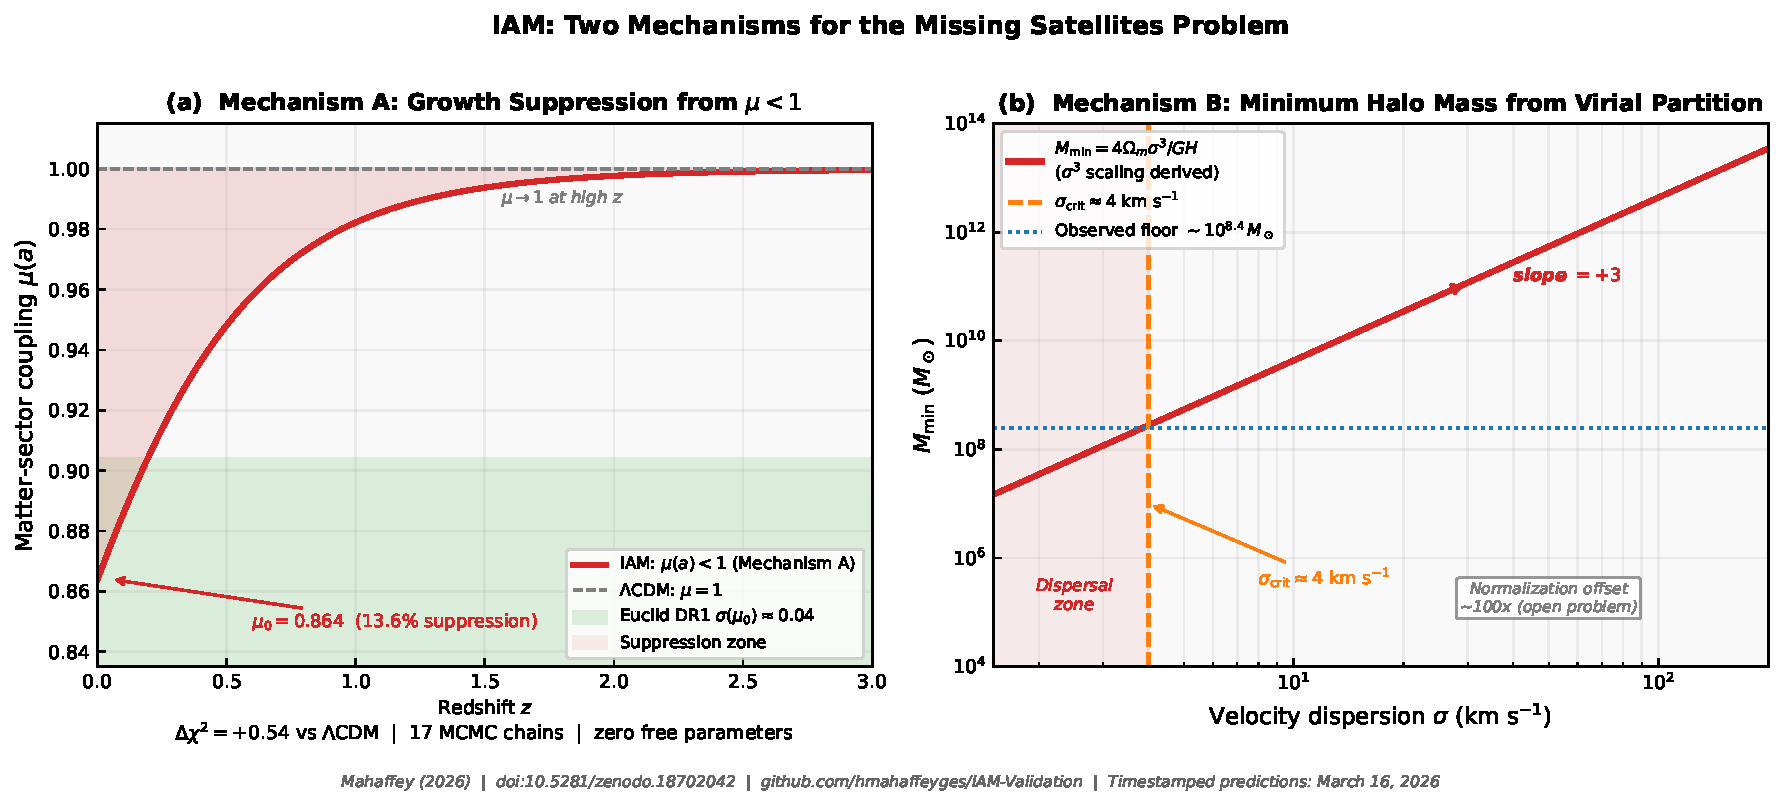
\includegraphics[width=0.94\textwidth]{iam_missing_sat_fig1.pdf}
\caption{The two IAM mechanisms. Panel~(a): Mechanism~A, the matter-sector
gravitational coupling $\mu(a)$ as a function of redshift. At $z = 0$,
$\mu_0 = 0.864$ (13.6\% suppression). At high $z$, $\mu \to 1$ and IAM
recovers $\Lambda$CDM behavior. The Euclid DR1 sensitivity band
($\sigma(\mu_0) \approx 0.04$) is shown. Result from 17 converged MCMC
chains against Planck~2018; $\Delta\chi^2 = +0.54$ versus $\Lambda$CDM.
Panel~(b): Mechanism~B, the minimum halo mass $M_\mathrm{min} = 4\Omega_m
\sigma^3/GH_0$ (Equation~\ref{eq:Mmin}) as a function of velocity dispersion.
The $\sigma^3$ scaling is derived with zero free parameters. The observed
halo occupation floor ($\sim 10^{8.4}\,M_\odot$, \citealt{Kim2021}) intersects
the predicted curve at $\sigma_\mathrm{crit} \approx 4$~km\,s$^{-1}$.
The normalization offset of $\sim$100$\times$ is an identified open problem.
Timestamped predictions established March~16, 2026.}
\label{fig:mechanisms}
\end{figure}

% ─────────────────────────────────────────────────────────────────────────────
\section{The Unified Picture}
\label{sec:unified}
% ─────────────────────────────────────────────────────────────────────────────

The two mechanisms operate simultaneously and address different aspects of the
satellite deficit. Mechanism~A suppresses the growth rate of all matter
perturbations at late times, reducing the abundance of dark matter halos
across the entire low-mass end of the mass function. This is a continuous
suppression operating from $z \sim 2$ to the present, controlled by a single
derived parameter $\beta_m = \Omega_m/2$.

Mechanism~B imposes a hard threshold. Below $\sigma_\mathrm{crit}$, halos
cannot close their virial partition; they disperse regardless of the growth
rate. This threshold is sharp in $\sigma$ and operates independently of
Mechanism~A.

Together, the mechanisms address the satellite deficit from two directions:
Mechanism~A reduces the number of halos that grow massive enough to host
satellites; Mechanism~B prevents halos below $\sigma_\mathrm{crit}$ from
virialization at all. Both derive from the same physical condition: the
virial partition must close on both channels simultaneously.

\begin{figure}[H]
\centering
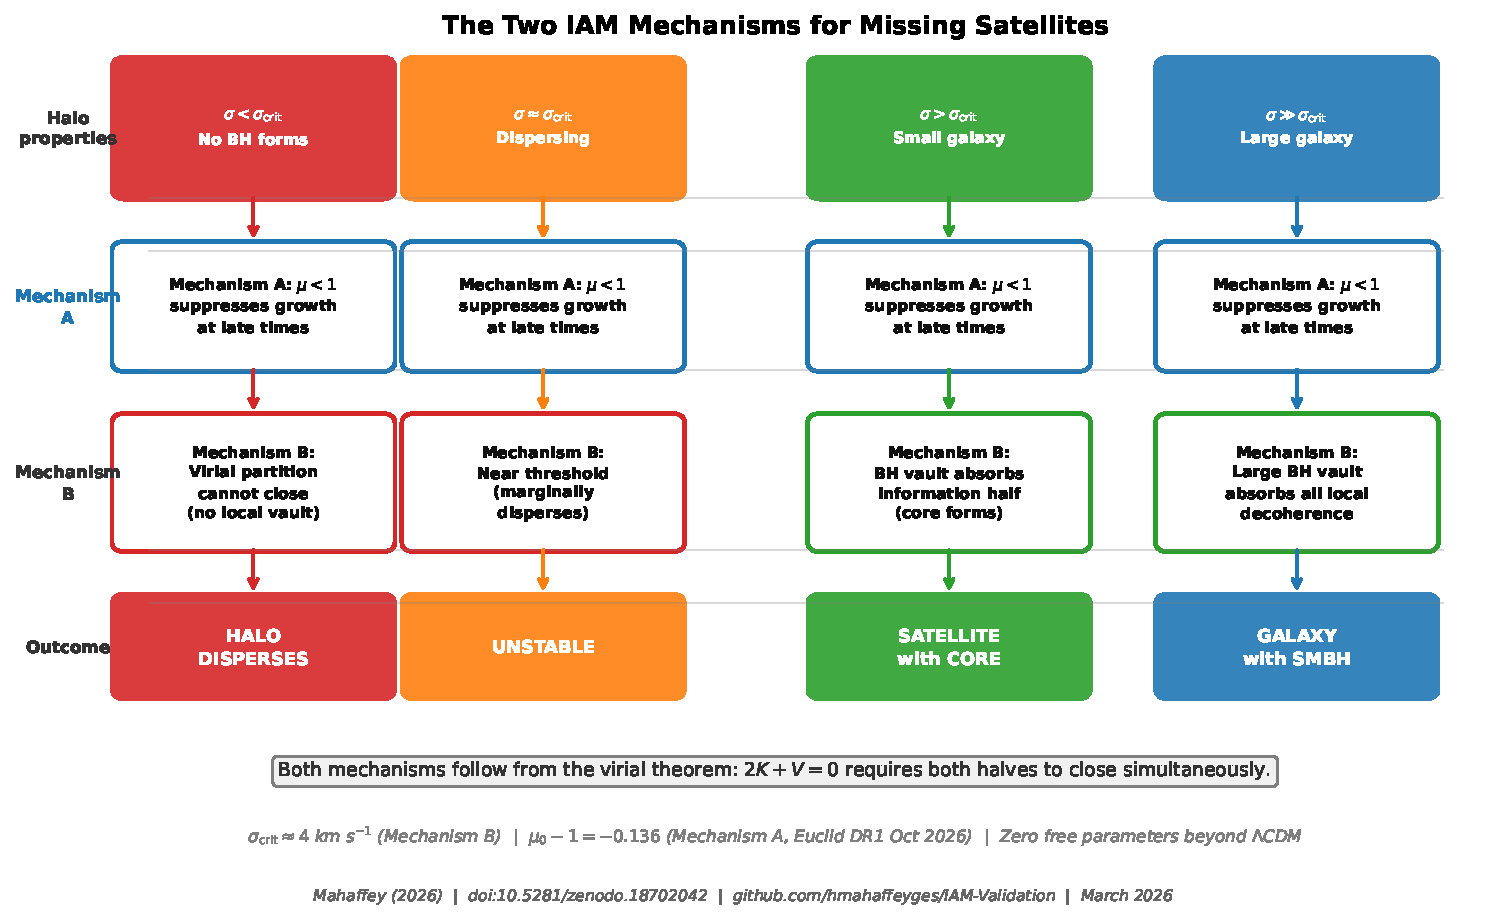
\includegraphics[width=0.90\textwidth]{iam_missing_sat_fig2.pdf}
\caption{The unified mechanism across four halo regimes. The virial partition
closure condition requires both halves of the virial partition to close
simultaneously. Mechanism~A ($\mu < 1$, confirmed by 17 MCMC chains) reduces
growth at late times for all halos. Mechanism~B (dispersal condition) imposes
a threshold below which no halo can virialize. Both mechanisms share the same
physical origin: $2K + V = 0$ at every scale.}
\label{fig:unified}
\end{figure}

This picture differs qualitatively from baryonic explanations. Reionization,
tidal stripping, and feedback all act on the baryon content of dark matter
halos that are assumed to have already virialized. The IAM mechanisms act
on the dark matter subhalo population itself: Mechanism~A by suppressing
growth, Mechanism~B by preventing virialization. The two classes of
explanation are not mutually exclusive; IAM suppression of the subhalo
population does not preclude baryonic processes also operating. However,
the IAM mechanisms are the only proposals that derive from the same
thermodynamic framework as the cosmological constant and the M--$\sigma$
relation, with the same zero free parameters.

% ─────────────────────────────────────────────────────────────────────────────
\section{Observational Tests and Falsification}
\label{sec:tests}
% ─────────────────────────────────────────────────────────────────────────────

The two mechanisms produce distinct, independently falsifiable predictions.

\textbf{Mechanism A.} The Euclid DR1 weak lensing survey (October 2026) will
measure $\mu_0$ to $\sigma(\mu_0) \approx 0.04$ precision~\citep{Euclid2024}.
IAM predicts $\mu_0 - 1 = -0.136$. This constitutes a $3.4\sigma$ detection
if correct, or a definitive exclusion if absent. The combined Euclid~+~DESI
Year~5 dataset will reach $5.4\sigma$ sensitivity~\citep{IAM_survey}. A
measurement of $\mu_0 > 0.90$ at $2\sigma$ would be in tension with the IAM
prediction.

\textbf{Mechanism B.} The Vera Rubin Observatory LSST will provide a
near-complete census of Milky Way satellite galaxies to limiting surface
brightness $\mu_V \approx 32$~mag\,arcsec$^{-2}$~\citep{LSST2009}. If the
satellite count continues to drop sharply below
$\sigma \approx 4$~km\,s$^{-1}$ as the survey depth increases, this is
consistent with the $\sigma_\mathrm{crit}$ prediction. If a significant
population of satellites below $\sigma_\mathrm{crit}$ is discovered, the
dispersal condition is inconsistent with observations and Mechanism~B requires
revision. The $\sigma^3$ mass--velocity scaling (Equation~\ref{eq:Mmin}) is
also independently testable: measurements of $M_\mathrm{min}$ as a function
of $\sigma$ for known dwarf spheroidals should follow a $\sigma^3$ trend.

\textbf{Cross-check.} The two mechanisms predict correlated suppression of
the power spectrum at the same scales. A joint measurement of $\mu_0$ from
Euclid and $\sigma_\mathrm{crit}$ from Rubin, combined with the
$\beta_m = \Omega_m/2$ prediction already confirmed at $0.2\sigma$ by
Planck~2018, would constitute a three-way consistency test of the virial
partition closure condition at cosmological and galactic scales simultaneously.

% ─────────────────────────────────────────────────────────────────────────────
\section{Discussion}
\label{sec:discussion}
% ─────────────────────────────────────────────────────────────────────────────

The missing satellites problem has been approached primarily as a problem of
baryonic physics: which processes remove gas from satellites, suppress star
formation, or disrupt dark matter halos after they form. The IAM framework
approaches it differently. The question is not what prevents baryons from
settling into subhalos, but what determines whether dark matter halos
virialize in the first place.

The answer, within IAM, is thermodynamic. A halo virializes when both halves
of the virial partition can close. The geometric half always finds its channel
in spacetime curvature. The informational half requires an available encoding
surface. At the satellite mass scale, that surface must be a local black hole
horizon. The minimum mass for black hole formation in a collapsing halo
determines the minimum mass for virialization. Below that mass, the partition
cannot close. The halo disperses. No satellite forms.

The open problem --- the normalization offset of $\sim$100$\times$ in
Equation~\ref{eq:Mmin} --- is identified precisely. It requires the formal
derivation of the local-to-global encoding rate criterion: the condition under
which decoherence events register on the local black hole horizon versus the
global cosmic horizon. This criterion involves the ratio of local to global
decoherence rates and the thermodynamic temperature differential between the
two horizons. Both quantities are calculable within IAM without additional
free parameters~\citep{IAM_BH}. The problem is identified here as an open
problem rather than a solved one.

The scaling predictions --- $\sigma^3$ for Mechanism~B, $\sigma^2$ for
cusp-core, $\sigma^4$ for M--$\sigma$ --- form a coherent family. All three
derive from the same thermodynamic identity~\citep{IAM_thermo_virial} at different boundary conditions. All
three have the same coupling constant $\beta_m = \Omega_m/2$. The different
power-law indices reflect different physical regimes: the minimum mass for
virialization (Mechanism~B), the encoding radius within a virialized halo
(cusp-core), and the steady-state SMBH mass accumulated over a Hubble time
(M--$\sigma$). A complete test of the virial partition closure condition requires
consistency across all three scalings simultaneously.

% ─────────────────────────────────────────────────────────────────────────────
\section*{Acknowledgments}
% ─────────────────────────────────────────────────────────────────────────────

The thermodynamic framework of T.\ Jacobson~\citep{Jacobson1995} is the
foundation upon which this work is built. Timestamped predictions for the
missing satellites problem and cusp-core scaling were established in the
GitHub repository on March~16, 2026, prior to the analysis presented here.

% ─────────────────────────────────────────────────────────────────────────────
\section*{Data Availability}
% ─────────────────────────────────────────────────────────────────────────────

All MCMC chains, analysis scripts, and timestamped prediction figures are
publicly archived at \url{https://github.com/hmahaffeyges/IAM-Validation}
with canonical Zenodo DOI
\href{https://doi.org/10.5281/zenodo.18702042}{10.5281/zenodo.18702042}.

% ─────────────────────────────────────────────────────────────────────────────
\bibliographystyle{plainnat}
\bibliography{iam_missing_satellites}
% ─────────────────────────────────────────────────────────────────────────────

\end{document}
